\chapter{Circuits combinatoires}
\minitoc
\section{Définition}
Un système numérique est dit combinatoire si toutes ses sorties, à tout instant $t$, ne dépendent que de la combinaison de
ses valeurs d'entrées et aucunement des sorties précédemment calculées. Les {\it systèmes combinatoires n'ont pas de mémoire d'un état interne passé}, alors que c'est le cas pour les systèmes séquentiels, caractérisé par cet état.
Notons que, dans le détail de la physique sous-jacente, les choses sont un peu plus compliquées :
on peut en effet noter que, même dans un circuit combinatoire, il existe un effet mémoire lié aux différentes mini-capacités
(condensateurs) qui sont susceptibles d'emmagaziner de l'énergie (sur les connexions etc). Ainsi les sorties dépendent des valeurs des entrées à un instant $t-\delta$
Toutefois, on sait que si l'on attend suffisamment longtemps, cet effet mémoire s'évanouit...\\

Il faut donc retenir l'intuition des systèmes combinatoires :
après avoir positionné des entrées, et lorsqu'on attend un temps suffisant (le $\delta$ de la définition),
on verra un résultat en sortie, qui ne dépend que des entrées (supposées stables)...

\section{Portes logiques de base}

Le tableau suivant résume les principales portes logiques dont nous ferons usage. Ces portes se présentent sous plusieurs formes équivalentes :
graphiques, équationnelles ou tabulées. Il faudra être à même de basculer d'une de ces représentations à une autre. Dans le tableau figurent deux types de
symboles : à gauche on trouve les symboles IEC, et à droite les symboles ANSI (dits "américains"). Les symboles IEC ne sont quasiment pas utilisés désormais, et
nous conseillons ici vivement de leur préférer les symboles américains. L'IEC reste utilisé dans le domaine du contrôle industriel, qui n'est qu'une infime partie de
l'Electronique traitée ici, dans sa généralité.

\begin{center}
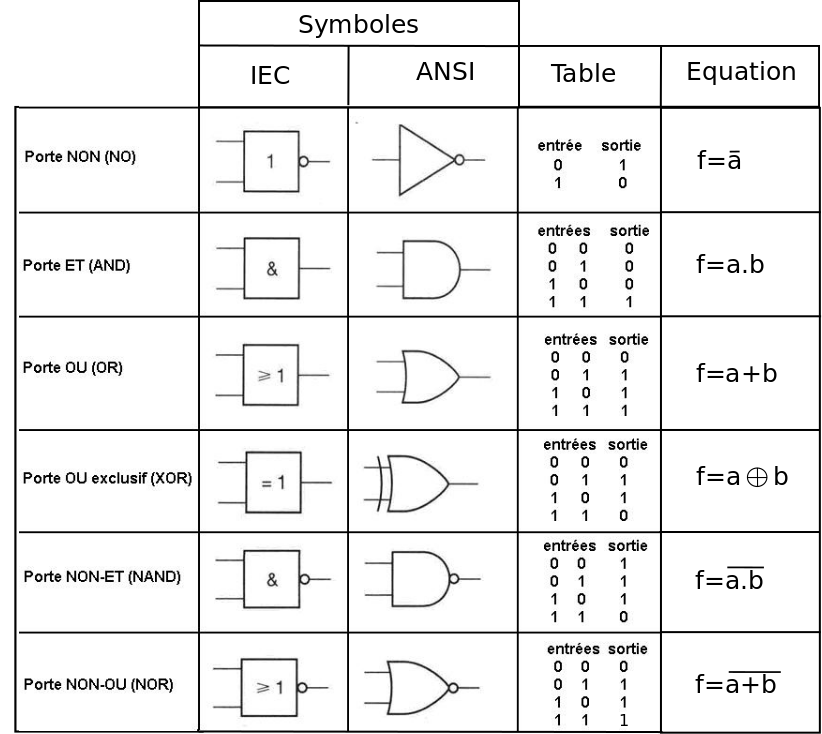
\includegraphics[scale=0.4]{./figures/table_verite.png}
\end{center}

\paragraph{Première approche : et, ou, non}
Les portes logiques de base reflètent directement les opérations élémentaires de l'algèbre de Boole : conjunction, disjonction et
négation. Ces portes permettent de construire directement un circuit électronique à partir d'une (ou plusieurs) expression(s) booléenne(s) donnée(s). L'assemblage
telles portes logiques (auquelles on ajoutera bientôt un élement séquentiel) forme une {\it netlist} (ou, en français, {\it liste d'interconnexions})
. Dans des cas réels, cette netlist peut contenir plusieurs millions de tels élements de base. A l'inverse, à partir d'un schéma de
netlist, il est possible de revenir à une ou plusieurs équations booléennes. Tout système numérique peut être envisagé comme tel : un vaste ensemble (graphe) de portes logiques.

\paragraph{Deuxième approche : autres portes logiques}
Dans la pratique, il est utile de pouvoir également disposer de portes logiques comme le XOR (ou exclusif), Nand, Nor à deux  entrées, mais également à plusieurs entrées (AND3, AND6 etc).
Technologiquement, ces portes complexes sont construites {\it à façon} par un {\it fondeur}. Parmi ces fondeurs, on trouve des sociétés comme STMicroelectronics, Samsung, Texas Instrument, IBM, TSMC, Intel etc.
Certaines d'entre elles ne produise de circuits que pour leur propre fabrication (Intel) tandis que d'autres (TSMC) permettent à une société tierce d'accéder à ces fonderies.

\paragraph{Troisième approche : non-et (nand)}

Une seconde manière de parler des portes logiques de base est de se pencher sur les propriétés de l'algèbre de Boole. On peut se rendre à l'évidence que les trois fonctions AND, OR et NOT
peuvent se calculer à l'aide d'une autre porte logique {\it unique}, qui devient ainsi la brique élémentaire de tout circuit numérique. Il s'agit de la porte NAND (non-et). Le calcul est également
possible avec le NOR, mais il est de tradition de considérer uniquement le NAND. Pour simplifier l'écriture, posons $\overline{a.b}=a \odot b$. On a donc $a \odot 1=not(a)$.
Prenons la formule $y=a+b$ et exprimons là à l'aide de $\odot$. Posons $\alpha=a$ et $\beta=b$.  On a donc :

\begin{align}
y &=  a + b \\
y  &= \overline{\alpha.\beta}\\
y  &= \alpha \odot \beta\\
y &= (a \odot 1) \odot (b \odot 1)
\end{align}

De même, on peut démontrer que :
\begin{align}
y &=  a.b \\
y  &= \overline{\alpha}.\overline{\beta}\\
\end{align}
d'où :
\begin{align}
\overline{y}  &=  \overline{\overline{\alpha}.\overline{\beta}}\\
  &=  a \odot b
\end{align}
et : $$y=(a \odot b) \odot 1$$

Il est donc possible d'exprimer toute la logique booléenne à l'aide du NAND, et ainsi construire n'importe quel circuit à l'aide de la porte logique NAND \footnote{Un livre d'introduction aux circuits profite de cette curiosité et s'intitule "Nand to Tertis"}.
Au dela de cette curiosité mathématique, il se trouve qu'en terme de transistors, il est plus facile de réaliser les portes NAND et NOR que des portes non complémentées.

\section{Fonctions logiques "complexes"}

\paragraph{Assemblage de portes logiques}

En s'en tenant au 3 portes logiques précédentes, on peut connecter les sorties des unes aux entrées des autres de manière à réaliser des fonctions de plus plus complexes, à l'image
de la fonction présentée en début de ce chapitre. Cet assemblage ne nécessite pas de précautions particulières, alors cela était nécessaire en électronique analogique (adapation d'impédance etc).
Il faudra toutefois veiller à ne pas "chaîner" un "trop" (cela reste à définir...) grand nombre de portes logiques les unes derrière les autres : bien que fonctionnellement correct, un tel assemblage
a tout lieu d'affecter la performance finale du circuit : nous allons en parler dans un paragraphe à suivre.

\paragraph{Notion de "Nuage combinatoire"}
Cet assemblage de portes logiques représente une fonction mathématique qui associe, à plusieurs entrées logiques, plusieurs sorties logiques. Nous allons rapidement
créer des fonctions logiques de plus en plus complexes : une fois qu'elles seront établies, {\it une bonne fois pour toutes}, il n'y aura plus lieu d'en étudier la structure.
Très rapidement, nous chercherons donc à {\it abstraire ces fonctions} : les langages de description matériel commme VHDL nous y aideront notamment, car de simples constructions
du langage permettront, en réalité, de "parler" de ces fonctions. Ainsi la simple addition numérique, constituée d'un grand nombre de porte logiques, sera simplement abstraite par le symbole "+", ce qui
est fort pratique ! De même, au lieu de décrire des multiplexeurs, on sera bientôt tenté de les substituer par un "if..then else" du langage. Mais sans en référer à VHDL, il est
parfois pratique de réaliser {\it graphiquement} ces fonctions : il n'est donc pas rare de remplacer la fonction numérique par un simple "nuage". Il s'agit d'un nuage "combinatoire".
L'assemblage d'"ordre supérieur" de tels nuages nous permettra de passer une autre échelle et concevoir des circuits encore plus complexes, en appliquant des "patterns" ou "motifs de conception".

\section{Mapping technologique sur circuits discrets}
Pendant longtemps, les ingénieurs disposaient de circuits {\it discrets}, se présentant sous la forme d'un boitier bien caractéristique, avec un nombre
de "pattes" (entrées et sorties) très limité (une dizaine). Pour concevoir un système, il s'agissait de sélectionner les bons boîtiers et de réaliser les soudures
apropriées pour effectuer la transition entre la netlist "théorique" et ces composants discrets. C'était un travail d'ingénieur des années 1970 et 80 !
A l'heure actuelle (2017) et depuis déjà bien longtemps, cette sélection se fait désormais par des algorithmes, au sein de programmes complexes (synthétiseurs logiques). Le nombre d'équations logiques, lui-même,
dépasse par ailleurs les capacités d'un être humain à les gérer. Surtout, ces composants discrets ont quasiment disparu, au profit de composants programmables (FPGA),
sur lesquels nous reviendront. Précisons que, sur ces composants programmables, le mapping
technologique garde tout son sens, puisqu'il s'agit encore de "mapper" une netlist théorique sur un ensemble de composants.

\begin{figure}[htb!]
  \centering
  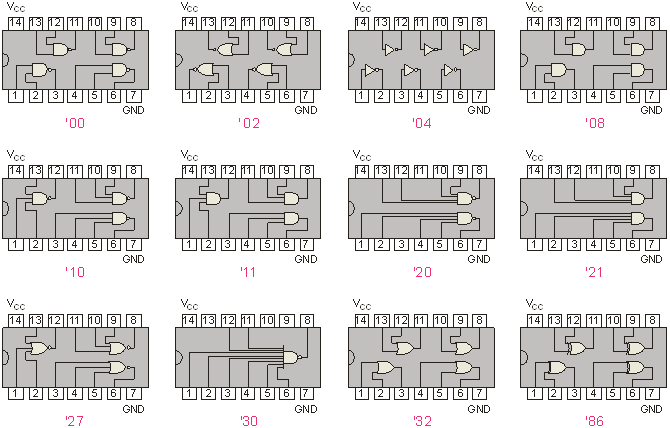
\includegraphics[width=10cm]{./figures/paste_image31.png}
  \caption{Exemple de circuits de la (mythique !) série 74, des années 70 et 80.}
\end{figure}


\section{Chemin critique et fréquence de fonctionnement}
La notion de chemin critique est d'une importance capitale. Il permet de calculer la fréquence maximale à laquelle on pourra soumettre un nouveau jeu d'entrées au circuit, sans perturber le calcul précédent. Cette fréquence
détermine {\it in fine} les performances finales de votre ordinateur.\\

Souvenons nous que, physiquement, nous avons affaire une interconnexion de composants, qui possèdent leurs propres resistance et capacité (et une inductance non significative). Un simple transistor possède un tel modèle équivalent...
Un signal électrique se présentant sur une entrée mettra un certain temps à agir sur les sorties du circuit : ce délai est directement relié à la capacité. Si on considère non plus une seule entrée, mais un ensemble d'entrées, la question que l'on peut se poser est la suivante : comment déterminer, parmi ces signaux, celui qui mettra le plus de temps
à se propager vers les sorties ? Pour cela, il suffit de parcourir la netlist et détecter {\it le plus long chemin entre les entrées et les sorties}.

Ce chemin est précisément le chemin combinatoire critique.
On fait généralement un abus de langage (toléré !) en associant ce chemin critique avec le {\it temps de propagation calculé sur ce chemin} : il faut connaître le temps caractéristique de traversée de chaque porte, ainsi que le temps de propagation sur chacun des fils qui les relient. En pratique,
des algorithmes calculent ce temps. Dès lors que l'on connait ce temps, on sait que c'est le laps de temps minimum pendant lequel, le circuit, {\it dans son intégralité}, ne pourra être utilisé pour un nouveau calcul. Si l'on possédait
un oscilloscope suffisamment précis, on pourrait constater, au cours de ce calcul, qu'une très grande agitation règne sur chacun des fils, et que cette agitation semble se propager des entrées vers les sorties, de manière anarchique.
Lorsque cette "vague" est passée, les fils de sortie se sont enfin stabilisés : on peut lire la sortie combinatoire. A l'inverse, si au cours de ce temps, on s'ingénie à vouloir utiliser la sortie, elle sera immanquablement fausse et instable.\\

Pour calculer la fréquence finale, on peut, {\it en première approximation} prendre l'inverse de ce temps \footnote{Nous verrons plus loin qu'il faut lui adjoindre deux autres composantes temporelles, liées aux bascules D}.
$$F_{max} \approx \frac{1}{t_{critic}}$$

\begin{center}
  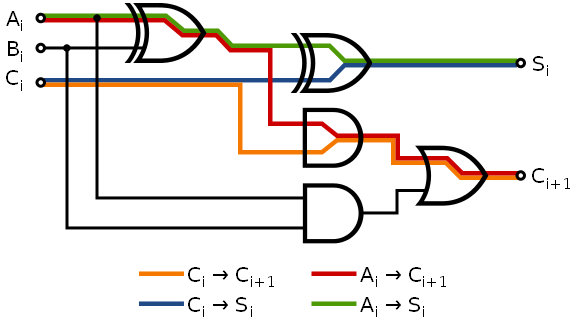
\includegraphics[width=6cm]{./figures/chemin-critique.png}
\end{center}

Cette "vague" fort complexe ne semble guère propice à l'élaboration de systèmes un tant soit peu élaborés...
Fort heureusement, nous serons rapidement en mesure de nous permettre d'"oublier" totalement ces phénomènes microscopiques, pour nous
concentrer sur l'essence des services macroscopiques que devra déliver notre système. Cette "libération" passe par la notion de circuits séquentiels.

\section{Arithmétique de base}
Nous abordons ici l'utilisation de portes logiques combinatoire afin d'élaborer des opérateurs de calculs "classiques" : additions d'entiers, multiplications etc.
On suppose d'emblée que l'on dispose d'{\it entrées} et de {\it sorties} numériques : il s'agit d'un ensemble de fils présentant (chacun) une tension 0 ou 5 Volts (selon la technologie, ces tensions peuvent varier).
Pour véhiculer deux opérandes A et B, il faut connaître la dynamique des valeurs que l'on veut traiter pour A et B : à partir de cette dynamique, on dispose d'un ensemble de fils
pour A et d'un ensemble de fils pour B, etc.

\subsection{Additionneur}
Il existe un grand nombre de manière d'assembler les portes logiques pour réaliser un calcul comme un additionneur.
La plus traditionnelle consiste à d'abord étudier le {\it demi-additionneur} (1 bit),
puis l' additionneur 1 bit {\it complet} (qui s'appuiera sur le demi-additionneur), puis chercher à étendre cet addition à des opérandes à plusieurs bits. Au coeur du procédé, on procède en utilisant le même algorithme
que celui enseigné dans notre enfance : on effectue une addition sur les digits les plus à droite, et on continue vers la gauche, en "marquant" d'éventuelles retenues.

\paragraph{Demi-additionneur 1 bit}
On parle de demi-additionneur afin de signifier qu'on ne s'intéresse pas, dans un premier temps, à la retenue entrante.
Le table de vérité et le circuits logique correspondant sont représentés ici. Les variables $s$ et $c$ dénotent la somme et la retenue (sortante).
Ce circuit s'appelle donc un demi-additionneur et est représenté par le symbole "HA" (half adder)
\begin{center}
   \begin{minipage}[t]{4cm}
     \vspace{0pt}
     \centering
     \begin{tabular}{|c|c||c|c|}
       \hline
       a & b & s & c \\ \hline
       0 & 0 & 0 & 0    \\ \hline
       0 & 1 & 1 & 0    \\ \hline
       1 & 0 & 1 & 0    \\ \hline
       1 & 1 & 0 & 1    \\ \hline
     \end{tabular}
   \end{minipage}%
   \begin{minipage}[t]{5cm}
     \vspace{0pt}
     \centering
     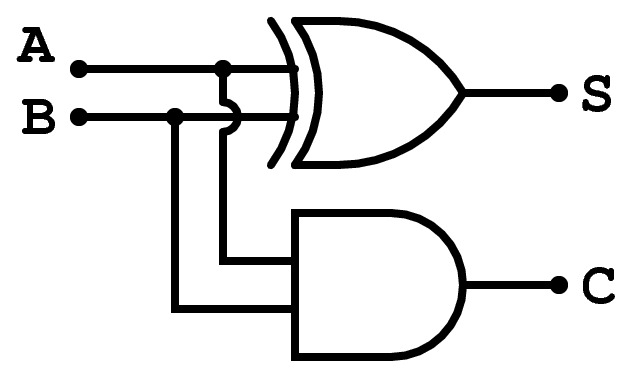
\includegraphics[width=3cm]{./figures/half_adder.jpg}
   \end{minipage}
   \begin{minipage}[t]{5cm}
     \vspace{0pt}
     \centering
     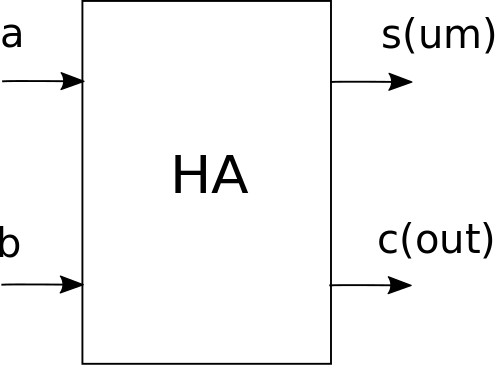
\includegraphics[width=3cm]{./figures/ha.png}
   \end{minipage}

\end{center} % added ending }



\paragraph{Additionneur 1 bit}

On introduit désormais la retenue entrante, afin de réaliser une addition sur n'importe quelle "colonne" de digits.
Un calcul permet de nous rendre compte que le demi-additionneur précédent peut être réutilisé. Il s'agit ici de notre premier
{\it assemblage hierarchique} de circuits.

\begin{center}
   \begin{minipage}[t]{4cm}
     \vspace{0pt}
     \centering
     \begin{tabular}{|c|c||c|c|c|}
       \hline
       a & b & $c_{in}$ & S & $C_{out}$ \\ \hline
       0 & 0 &   0 & 0 &         0 \\ \hline
       0 & 0 &   1 & 1 &         0  \\ \hline
       0 & 1 &   0 & 1 &         0  \\ \hline
       0 & 1 &   1 & 0 &         1  \\ \hline
       1 & 0 &   0 & 1 &         0 \\ \hline
       1 & 0 &   1 & 0 &         1  \\ \hline
       1 & 1 &   0 & 0 &         1  \\ \hline
       1 & 1 &   1 & 1 &         1  \\ \hline

     \end{tabular}
   \end{minipage}%
   \begin{minipage}[t]{5cm}
     \vspace{-5pt}
     \centering
     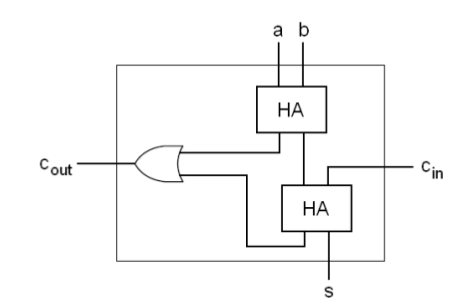
\includegraphics[width=5cm]{./figures/add-5.png}
   \end{minipage}
   \begin{minipage}[t]{5cm}
     \vspace{0pt}
     \centering
     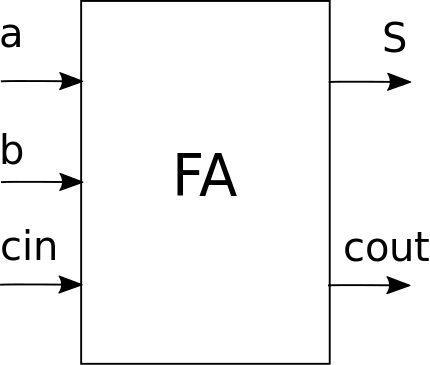
\includegraphics[width=3cm]{./figures/full_adder.png}
   \end{minipage}
\end{center} % added ending }

Le calcul évoqué est exposé ici. Au préalable on établit l'égalité suivante où $\oplus$ représente le {\it ou exclusif}:
$$\barre{a\oplus b}=\barre{a.\barre{b}+\barre{a}.b}=(\barre{a}+b).(a+\barre{b})=\barre{a}.\barre{b}+a.b$$
On a désormais :
\begin{align}
S  &= a.\barre{b}.c_i + a.b.c_i + a.\barre{b}.c_i + a.b.c\\
   &= a.(a\oplus c_i) + a (b\oplus c_i)\\
   &= a \oplus b \oplus c_i
\end{align}
De même, on trouve : $c_o=a.b+(a\oplus b).c_i$.
Le demi additionneur peut donc effectivement être ré-utilisé judicieusement, comme dessiné sur la figure précédente.

\paragraph{Additionneur {\it n} bits}
La manière la plus naturelle (mais pas la plus efficace !) consiste à chaîner les retenues sortantes et entrante : on parle d'{\it additionneur à propagation de retenue} ou {\it Ripple-carry Adder}.
Nous présentons ici un additionneur 4 bits avec retenue entrante. En général cette retenue est fixée à 0, mais nous verrons un peu plus loin qu'elle peut également être très utile. En exercice, on peut tenter de déterminer le chemin critique de ce circuit (l'exercice
est moins trivial qu'il n'y parait...).
\begin{center}
  \centering
  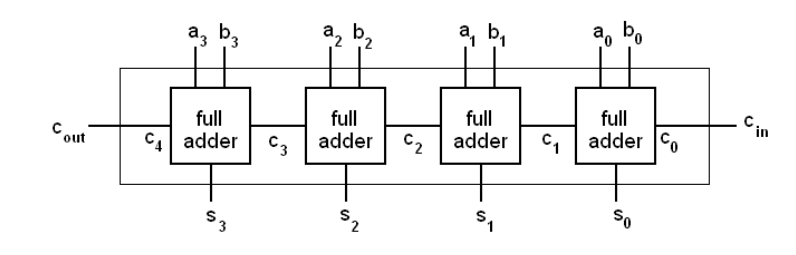
\includegraphics[width=9cm]{./figures/add-6-rc.png}
\end{center}

\subsection{Soustracteur}
Cherchons désormais les équations du soustracteur logique.
\paragraph{Utilisation d'une table de vérité}
On procède de même que précédemment, en écrivant la table de vérité du demi-soustracteur (HS), puis aux équations logiques. Sans surprise, ces équations
ressemblent de très près à celle du demi-additionneur : en numérique aussi, l'addition et la soustraction sont des opérations similaires.
On remarque l'adjonction d'un unique inverseur dans le calcul de la retenue sortante.
\begin{center}
   \begin{minipage}[t]{4cm}
     \vspace{0pt}
     \centering
     \begin{tabular}{|c|c||c|c|}
       \hline
       a & b & D & c \\ \hline
       0 & 0 & 0 & 0    \\ \hline
       0 & 1 & 1 & 1    \\ \hline
       1 & 0 & 1 & 0    \\ \hline
       1 & 1 & 0 & 0    \\ \hline
     \end{tabular}
   \end{minipage}%
   \begin{minipage}[t]{8cm}
     \vspace{5pt}
     \centering
     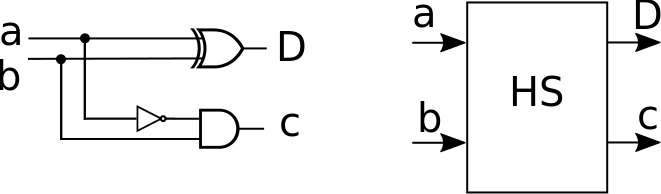
\includegraphics[width=8cm]{./figures/half_sub.png}
   \end{minipage}
\end{center} % added ending }
On pourrait procéder exactement de la même manière que nous l'avons fait pour établir la structure du soustracteur complet. Toutefois, nous n'allons pas
le faire ici, mais passer plutôt à l'utilisation du complément à 2.

\paragraph{Utilisation du complément à 2}
On sait en effet qu'algébriquement on a : $a-b=a+(-b)$. On peut donc voir la soustraction comme une addition de deux nombres dont le second est l'{\it inverse de $b$}.
Attention ! Nous parlons d'"inverse" dans l'algèbre des nombres entiers, mais nous savons désormais (voire le premier chapitre) que $-b$ doit se représenter en complément à 2 en logique
booléenne.
Il faut donc procéder en inversant les entrées $b_i$ et en ajoutant '1' : cet ajout se fait par la retenue entrante, dont on saisit désormais l'intérêt.
\begin{center}
  \centering
  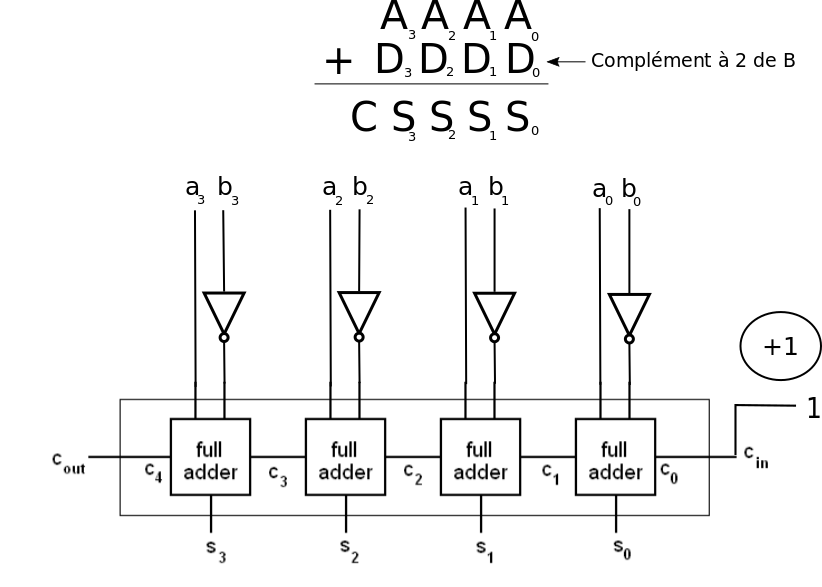
\includegraphics[width=9cm]{./figures/soustracteur.png}
\end{center}


\subsection{Additionneur-soustracteur}
Désormais munis d'additionneurs et de soustracteurs, nous pouvons nous pencher sur d'autres circuits intéressants. Avant d'aborder la mulitplication, étudions l'additionneur-soustracteur.
Comme son nom l'indique,il s'agit d'un circuit capable de réaliser, à volonté, soit l'addition, soit la soustraction. Il s'agit donc par là de notre premier circuit {\it programmable}, qui
nous rapproche au passage d'un ordinateur classique : selon le programme, considéré comme extérieur au processeur (il est stocké dans une mémoire séparée) qui s'exécute, c'est tantôt tel opérateur numérique qui opère, tantôt tel autre.
Dans le cas de l'additionneur-soustracteur, on procède par la même observation que la soustraction précédemment étudiée : quelles entrées $d_i$ dois-je fournir à l'additionneur ?
Dans le cas où je souhaite réaliser l'addition, on doit avoir $d_i=b_i$ (les $a_i$ restent bien évidemment inchangés), alors que pour la soustraction $d_i=\barre{b_i}$, sans oublier l'introduction d'un '1' sur
la retenue entrante.
Pour rendre commandable l'opération, on doit disposer d'une entrée supplémentaire, ici appelée "sub" : quand $sub=1$, le circuit effectuera la soustraction, et l'addition
dans l'autre cas. Etablissons les équations logiques des $d_i$ :
\begin{center}
   \centering
   \begin{tabular}{|c|c||c|}
     \hline
     $b_i$ & sub &  $d_i$ \\ \hline
         0 &   0 &  0    \\ \hline
         0 &   1 &  1    \\ \hline
         1 &   0 &  1    \\ \hline
         1 &   1 &  0    \\ \hline
   \end{tabular}
\end{center}
On voit que l'on a affaire à un magnifique "ou exclusif" ! $$d_i=b_i \oplus sub$$. Le schéma se réduit donc au suivant. Notons que l'introduction du '1' en retenue entrante correspond à la commande "sub".
\begin{center}
  \centering
  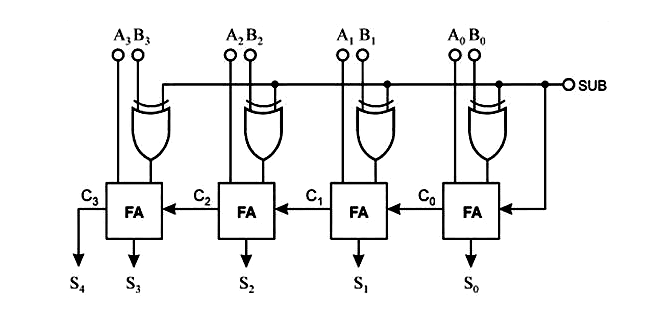
\includegraphics[width=9cm]{./figures/sub-2.png}
\end{center}

\subsection{Multiplieur}
\paragraph{Méthode naturelle}

Pour impléménter un multiplieur en logique combinatoire, il faut simplement comprendre ce qui se passe lorsqu'on "pose" une multiplication traditionnelle et reporter
le principe en respectant la logique booléenne. Le produit de 13 par 11 est donné ici en exemple.

\begin{center}
  \centering
  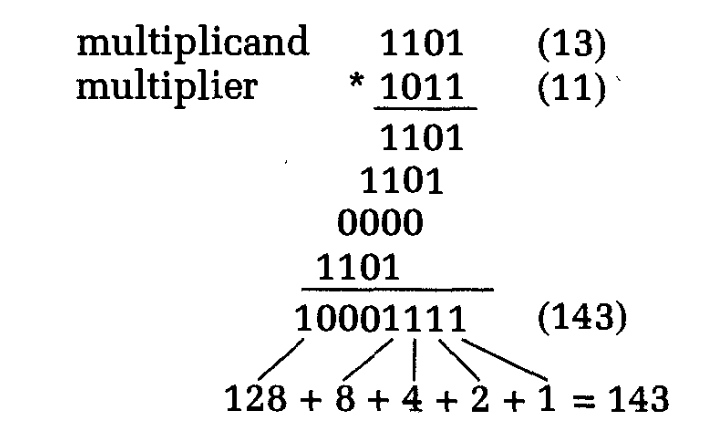
\includegraphics[width=5cm]{./figures/mult-1.png}
\end{center}

On se convainct facilement que la multiplication se réduit, ligne par ligne,
à un conjonction booléenne (et logique). Ligne à ligne, il faut ensuite additionner soit deux opérandes (demi-additionneur), soit trois lorsqu'une retenue est possible (full adder 1 bit).


\begin{center}
  \centering
  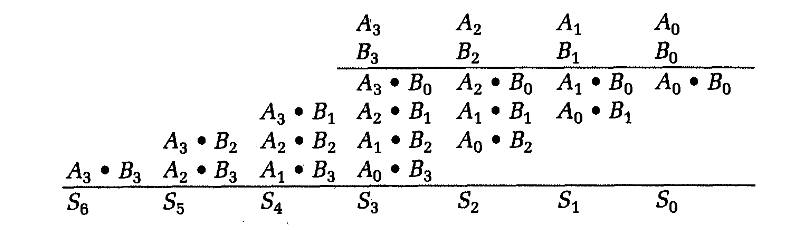
\includegraphics[width=9cm]{./figures/mult-2.png}
\end{center}

Etonnamment, le schéma \footnote{dû à Randu Katz, dont on pourra consulter le livre \cite{katz}} se révèle très irrégulier.

\begin{center}
  \centering
  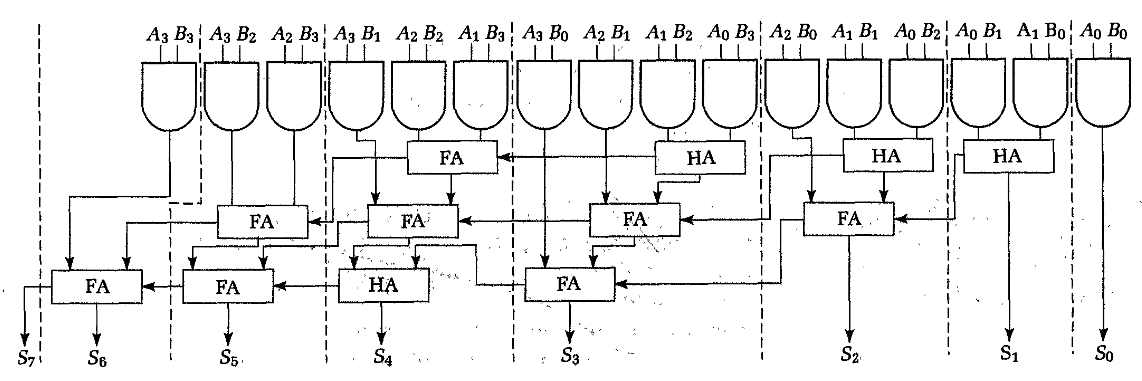
\includegraphics[width=9cm]{./figures/mult-3.png}
\end{center}

\paragraph{Multiplieur avec topologie régulière}
On peut chercher à réaliser un multiplieur, en cherchant un circuit élémentaire "brique de base", que l'on aboute savemment, mais de manière parfaitement régulière, en 2 dimensions. Les microélectroniciens aprécient particulièrement
ce type de circuits, qui se placent facilement sur silicium. Une tel circuit est donné ici à titre de curiosité.

\begin{center}
  \centering
  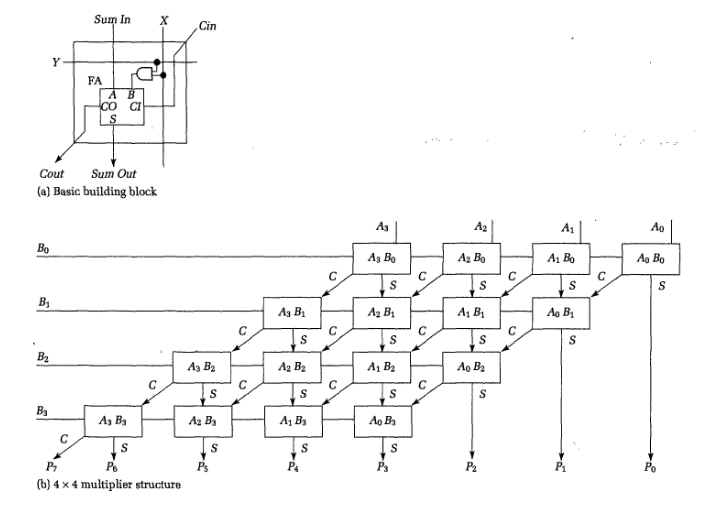
\includegraphics[width=9cm]{./figures/mult-4.png}
\end{center}

\subsection{Diviseur}
Le diviseur est un peu plus complexe. On repart là aussi de la division classique. Lors du calcul de $A/B$,
on soustrait le diviseur B de manière répétitive aux bits du dividende A, après l'avoir multiplié par '1' ou '0'.
Ce bit de multiplication '0' ou '1' est sélectionné pour chaque étape de soustraction de telle manière que le résultat
de la soustraction n'est jamais négatif. Le résultat est composé des bits de multiplication successifs, alors que
le reste est le résultat de la dernirèe soustraction. Cette algorithme combinatoire peut-être implémenté
comme une série de soustraction. Chaque soustracteur calcule la différence entre 2 nombres en entrée, mais
si le résultat est négatif, l'opération est annulée et remplacée par une soustraction de 0.

\section{Shifter}

\paragraph{Shifter à position fixe}
{\it Shift} signifie "décaler" en anglais. L'opération $f$ consiste à décaler, à droite ou à gauche, les bits $x_i$ de l'unique entrée $x$ présentée en entrée.
Le décalage d'un nombre fixe $\Delta$ de positions est tel que $y_i=f(x_i)=x_{i-\Delta}$. On décale à gauche pour $\Delta>0$ et à droite sinon. Cette opération sur
les seuls indices a la particularité de ne nécessiter {\it aucune} porte logique : il s'agit simplement de prendre un fil d'entrée et
de le connecter sur le bon fils de sortie. C'est une économie en silicium conséquente.

Le shifter à position fixe a notamment la particularité d'être d'une très grande utilité lorsque $\Delta$ est une puissance de 2. En effet,
décaler à gauche (resp. à droite) d'une position $\Delta$ revient à multiplier (resp. diviser) par $log_2(\Delta)$. Par exemple,
pour multiplier un nombre par 2 (resp. par 4,8,16 etc), il suffit, en binaire, de le décaler à gauche d'une position $\Delta=1$ (resp. $\Delta=2,3,4$ etc).
Alors que le multiplieur coûte cher en portes logiques, la cas de la multiplication par de telles puissances de 2 ne coûte rien.
\footnote{Dans le jeu d'instruction d'un processeur, cela a-t-il un intérêt ? La réponse est clairement oui, car il faut parfois plusieurs cycles d'horloges
pour attendre le résultat d'un multiplieur, afin de laisser au multiplieur (éventuellement totalement combinatoire) le temps d'effectuer son calcul.
A l'inverse, le shift est quasi immédiat et ne nécessite donc qu'un seul cycle machine. Nous y reviendrons...}

\paragraph{Barrel shifter}
Lorsque le nombre $\Delta$ n'est pas fixé, mais devient une entrée dur circuit, il faut être à même de décaler "à volonté".
Cette opération plus délicate nécessite un réseau de multiplexeurs.

\section{Multiplexeur}
Le multiplexeur a comme fonction de {\it router} une de ses entrées $e_i$ vers l'unique sortie $f$, en fonction d'une commande $c$.
La commande $c$ indique quelle $e_i$ doit effectivement passer. Mathématiquement cela peut s'écrire : $f(\{e_i,i \in 0..n-1\},c)=e_{c}$.
Il faut donc $\lceil(\log_2{n})$ bits pour constituer le mot de contrôle $c$.
Mais calculons simplement sa table de vérité dans le cas de 2 entrées ($a=e_0$ et $b=e_1$) et d'une commande $c$ (sur un seul bit) :
\begin{center}
   \begin{minipage}[t]{4cm}
     \vspace{0pt}
     \centering
     \begin{tabular}{|c|c|c||c|}
       \hline
       $a$ & $b$ &  c  &  f \\ \hline
       0 & 0 &  0  &  0 \\ \hline
       0 & 0 &  1  &  0 \\ \hline
       0 & 1 &  0  &  0 \\ \hline
       0 & 1 &  1  &  1 \\ \hline
       1 & 0 &  0  &  1 \\ \hline
       1 & 0 &  1  &  0 \\ \hline
       1 & 1 &  0  &  1 \\ \hline
       1 & 1 &  1  &  1 \\ \hline
     \end{tabular}
   \end{minipage}%
   \begin{minipage}[t]{5cm}
     \vspace{5pt}
     \centering
     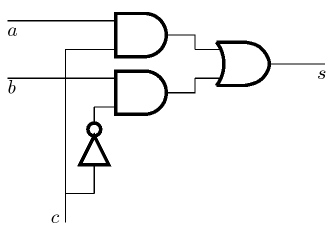
\includegraphics[width=4cm]{./figures/mux.png}
   \end{minipage}
   \begin{minipage}[t]{5cm}
     \vspace{0pt}
     \centering
     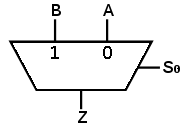
\includegraphics[width=3cm]{./figures/mux2to1.png}
   \end{minipage}
\end{center} % added ending }


Le multiplexeur est un des éléments clés de l'émulation d'une certaine intelligence
par du hardware : il permet de filtrer et d'acheminer des données vers un calcul (ou un élement de stockage), selon le calcul de certains critères transformés
en commandes de ces multiplexeurs. Ils seront logiquement un élément clé de la notion de {\it datapaths} ou "chemins de données", constitutifs de la partie calculatoire
d'un processeur, l'autre partie étant précisément la partie contrôle, et l'ensemble pouvant être interdépendant (un contrôle pouvant dépendre d'un calcul etc).

\paragraph{Crossbar}


\section{Comparateur}
Le comparateur participe souvent aux décisions évoquées à l'instant.

\paragraph{Comparateur 1 bit}
Etudions tout d'abord le comparateur entre 2 entrées $a$ et $b$ codées sur 1 bit.
Calculons les 3 fonctions $<$, $=$ et $>$.
\begin{center}
   \begin{minipage}[t]{4cm}
     \vspace{0pt}
     \centering
     \begin{tabular}{|c|c||c|c|c|}
       \hline
       a & b & $<$ & $=$ & $>$ \\ \hline
       0 & 0 &  0  &  1  & 0   \\ \hline
       0 & 1 &  1  &  0  & 0   \\ \hline
       1 & 0 &  0  &  0  & 1   \\ \hline
       1 & 1 &  0  &  1  & 0   \\ \hline
     \end{tabular}
   \end{minipage}%
   \begin{minipage}[t]{9cm}
     \vspace{-5pt}
     \centering
     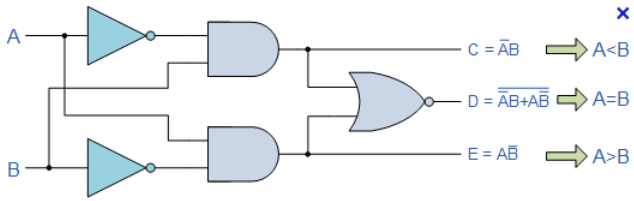
\includegraphics[width=8cm]{./figures/comparator-1.png}
   \end{minipage}
\end{center} % added ending }

\paragraph{Comparateur d'égalité de 2 entiers}
Pour passer à une comparaison d'égalité de 2 entiers $a$ et $b$ codés sur $n$ bits, il suffit
de les comparer bit à bit et s'assurer que chacune des comparaisons vaut bien '0'. Cela peut s'écrire :
$$Eq(a,b)=\prod_{i=0}^{i=n-1} a_i \oplus b_i$$
Le circuit dans le cas de $n=4$ est donné sur la figrue suivante.
\begin{center}
  \centering
  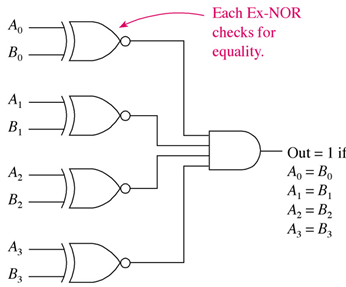
\includegraphics[width=6cm]{./figures/comparator-2.png}
\end{center}

\section{Codeurs et Décodeurs}

La fonction d'un codeur est la suivante : il transmet en sortie le code d'un symbole placé en entrée. Généralement ce code
est optimisé et plus simple à transmettre que le symbole initial. Par exemple, à partir de 3 symboles "bleu", "blanc", "rouge", il est
possible de ne transmettre que 2 bits établis au préalable par la fonction de codage : par exemple "00","01","10". A l'inverse, le décodeur
permettra par exemple de n'allumer qu'une des 3 couleurs "bleu", "blanc" et "rouge" à la réception de 2 bits.
\begin{center}
   \begin{minipage}[t]{4cm}
     \vspace{5pt}
     \centering
     \begin{tabular}{|c||c|c|}
       \hline
       couleur & $f_1$ & $f_0$ \\ \hline
       bleu    &    0  &     0 \\ \hline
       blanc   &    0  &     1 \\ \hline
       rouge   &    1  &     0 \\ \hline
     \end{tabular}
   \end{minipage}%
   \begin{minipage}[t]{9cm}
     \vspace{0pt}
     \centering
     \begin{tabular}{|c|c||c|c|c|}
       \hline
       $f_1$ & $f_0$ & bleu & blanc & rouge \\ \hline
          0  &     0 & 1 & 0 & 0 \\ \hline
          0  &     1 & 0 & 1 & 0 \\ \hline
          1  &     0 & 0 & 0 & 1 \\ \hline
          0  &     0 & 0 & 0 & 0 \\ \hline
     \end{tabular}
   \end{minipage}
\end{center} % added ending }

\paragraph{Décodeur 7-segments}
Parmi les décodeurs fréquemment utilisés, on trouve le décodeur 7-segments. Un afficheur 7 segments se présente comme un ensemble de 7 leds a,b,c,d,e,f,g
que l'on peut alumer ou éteindre individuellement. Nous calculerons en TD les 7 équations logiques associées pour les nombres hexadécimaux allant de 0 à 15.
\begin{center}
  \centering
  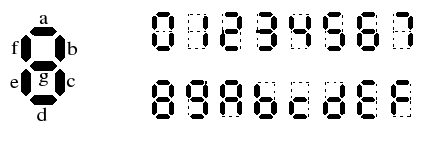
\includegraphics[width=6cm]{./figures/afficheur-7seg.png}
\end{center}

\section{Conclusion}
Ce chapitre a permis de nous familiariser avec un certain nombre de fonctions combinatoires usuelles. Leur caractère combinatoire s'est manifesté par le fait qu'à aucun moment, il n'a été nécessaire, au cours
des calculs menés, de se référer au passé des signaux en présence. Le calcul s'est toujours réalisé des entrées vers les sorties, sans retour possible.
Parmi les fonctions combinatoires intéressantes, l'arithmétique figure en bonne place. Souvenons nous que c'est bien par ces procédés que nous sommes en mesure
d'utiliser un matériau (le silicium ici) pour calculer ! Il faut savoir que le domaine de l'arithmétique sur silicium est un domaine toujours actif. Il est notamment
toujours à l'honneur dans le domaine de la cryptographie et des télécommunications en général.
On complètera la lecture de ce chapitre par la consulation d'autres ouvrages comme \cite{mano},\cite{clements}.
